\documentclass[12pt]{article}
\usepackage[top=2cm, left=3cm, right=3cm]{geometry}
\usepackage[utf8]{inputenc}
\usepackage[english]{babel}
\usepackage{times}
\usepackage{calc}
\usepackage{eso-pic}
\usepackage{titlesec}
\usepackage{array}
\usepackage{makecell}
\usepackage{graphicx}
\usepackage{tikz-uml}
\usepackage{pgfgantt}

\date{06 Oct, 2024}
\title{Cloud Maker}
\author{Vikas Kushwaha}

\nonstopmode

\newlength{\PageFrameTopMargin}
\newlength{\PageFrameBottomMargin}
\newlength{\PageFrameLeftMargin}
\newlength{\PageFrameRightMargin}

\setlength{\PageFrameTopMargin}{1cm}
\setlength{\PageFrameBottomMargin}{1cm}
\setlength{\PageFrameLeftMargin}{1cm}
\setlength{\PageFrameRightMargin}{1cm}

\makeatletter

\let\inserttitle\@title
\let\insertauthor\@author
\let\insertdate\@date

\newlength{\Page@FrameHeight}
\newlength{\Page@FrameWidth}

\AddToShipoutPicture {
	\thicklines
	\setlength{\Page@FrameHeight}{\paperheight-\PageFrameTopMargin-\PageFrameBottomMargin}
	\setlength{\Page@FrameWidth}{\paperwidth-\PageFrameLeftMargin-\PageFrameRightMargin}
	\put(\strip@pt\PageFrameLeftMargin,\strip@pt\PageFrameTopMargin){
		\framebox(\strip@pt\Page@FrameWidth, \strip@pt\Page@FrameHeight){}}}

\makeatother

\titleformat{\section}
{\Large\bfseries\center\uppercase}
{}
{1em}
{}
[\hrule]

\titleformat{\subsubsection}
{\bfseries\uppercase}
{\hspace{-0.5cm}}
{1em}
{}

\AddToHook{cmd/section/before}{\clearpage}
% \tikzumlset{fill usecase=white}
\graphicspath{ {./images/} }

\newenvironment{changemargin}[2]{%
\begin{list}{}{%
\setlength{\topsep}{0pt}%
\setlength{\leftmargin}{#1}%
\setlength{\rightmargin}{#2}%
\setlength{\listparindent}{\parindent}%
\setlength{\itemindent}{\parindent}%
\setlength{\parsep}{\parskip}%
}%
\item[]}{\end{list}}

\renewcommand\theadfont{\bfseries}
\newcolumntype{L}[1]{>{\raggedright\let\newline\\\arraybackslash\hspace{0pt}}m{#1}}
\newcolumntype{C}[1]{>{\centering\let\newline\\\arraybackslash\hspace{0pt}}m{#1}}
\newcolumntype{R}[1]{>{\raggedleft\let\newline\\\arraybackslash\hspace{0pt}}m{#1}}


\begin{document}

\begin{center}
	\fontsize{14pt}{28pt}\selectfont
	A PROJECT REPORT \\
	on \\
	\textbf{"\underline{\MakeUppercase{\inserttitle}}"} \\
	\textit{submitted by} \\
	\textbf{Mr. \insertauthor} \\
	\textbf{Seat No :-} \\
	\textit{in partial fullfillment for the award of the degree} \\
	of \\
	\textbf{BACHELOR OF SCIENCE} \\
	in \\
	\textbf{COMPUTER SCIENCE} \\
	\textit{under the guidance of} \\
	\textbf{Mrs. Swetha Iyer} \\
	\textbf{Department of Computer Science} \\
	\vspace{1cm}
	
\includegraphics[scale=0.25]{vartak-logo} \\
	\fontsize{14pt}{20pt}\selectfont
	\textbf{VIDYAVARDHINI'S} \\
	\textbf{A. V. COLLEGE OF ARTS, K. M. COLLEGE OF COMMERCE} \\
	\textbf{E. S. A. COLLEGE OF SCIENCE,} \\
	\textbf{VASAI(WEST), PALGHAR-401208, MAHARASHTRA} \\
	\fontsize{14pt}{28pt}\selectfont
	\textbf{(Sem V)} \\
	\textbf{(2024-25)} \\
\end{center}


\fontsize{12pt}{24pt}\selectfont

\section{Acknowledgement}
\begin{center}
	\vspace{2cm}
	I would like to acknowledge my sincere thanks towards our project guide \\
	\textbf{Head of Computer Scince Department} \\
	\textbf{Mrs. Srimathi Narayanan} \\
	for their valuable guidance and suggestions and \\
	providing me an opportunity to do the project work in the college lab and \\
	which made me complete the project successfully. \\
	\vspace{2cm}
	I am also thankful to \\
	\textbf{Mrs. Gyaneshwari Pawar} \\
	For providing such nice guidance in form of comments and corrections. \\
	I am thakful to and fortunate enough to get contant encouragement, \\
	support and guidance from all teaching staff of Computer Science \\
	which helped us in successfully completing our project work. \\
Also, I would like to extend our sincere esteems to all staff in laboratory \\
	for their timely support. \\
	\vspace{2cm}
	By \textbf{\insertauthor}, \\
	T.Y.BSc (Computer Science)
\end{center}


\section{Declaration}
\vspace{2cm}
I \textbf{\underline{\insertauthor}} hereby declare that, \\
\bigskip \\
The project entitled
\textbf{"\underline{\MakeUppercase{\inserttitle}}"}
submitted in the partial fulfillment for the award of Bachelor of Science in Computer Science during the academic year \textbf{2023 - 2024} is my original work and the project has not formed the basis for the award of any degree, associate ship, fellowhip or any other similar titles. \\ \\ \\
\vspace{2cm}
\textbf{Signature of the Student:} \\
\bigskip
\textbf{Place:} \\
\bigskip
\textbf{Date:} \\


\section{Plagarism Report}


\section{Gantt Chart}


\section{Table Of Content}
\vfill
\begin{center}
\begin{tabular}{ | C{2cm} | m{8cm} | C{2cm} | m{2cm} | }
	\hline
	\thead{Sr. No} & \thead{Contents} & \thead{Page No.} & \thead{Sign} \\
	\hline
	\hline\textbf{1.}  & \textbf{Introduction} & \textbf{} & \\
	\hline\textbf{2.}  & \textbf{Limitation of Current System} & \textbf{} & \\
	\hline\textbf{3.}  & \textbf{Advantages of Proposed System} & \textbf{} & \\
	\hline\textbf{4.}  & \textbf{Tools and Techniques} & \textbf{} & \\
	\hline\textbf{5.}  & \textbf{Requirement Specification} & \textbf{} & \\
	\hline\textbf{6.}  &
	\bgroup
	\def\arraystretch{0.7}%
	\begin{tabular}{L{0.7cm} l}
		& \textbf{System Design} \\
		\textbf{(A)} & Event Table \\
		\textbf{(B)} & ER Diagram \\
		\textbf{(C)} & Class Diagram \\
		\textbf{(D)} & Use Case Diagram \\
		\textbf{(E)} & Sequence Diagram \\
		\textbf{(F)} & Component Diagram \\
		\textbf{(G)} & Deployment Diagram \\
		\textbf{(H)} & Activity Diagram \\
		\textbf{(I)} & Database \\
	\end{tabular}
	\egroup
		& \textbf{} & \\
	\hline\textbf{7.}  & \textbf{System Implementation} & \textbf{} & \\
	\hline\textbf{8.}  & \textbf{Results} & \textbf{} & \\
	\hline\textbf{9.}  & \textbf{Conclusion} & \textbf{} & \\
	\hline\textbf{10.} & \textbf{References} & \textbf{} & \\
	\hline
\end{tabular}
\end{center}
\vfill


\section{Introduction}
\vspace{1cm}
\textbf{\ul\uppercase{Title of the Project:}} \quad\textbf{\MakeUppercase{\inserttitle}}
\bigskip
\subsubsection{Synopsis:} \quad\quad
\textit{A cloud storage in distributed fashion.} \\ \par
This system is intended to be an alternative to online storage proveders like Google Drive. It's a distributed model where the user physically owns the resources in his/her own house. Unlike centralised cloud providers, the user is given a small computing device, preferrably an SBC like Rasberry Pi which acts as an 'Endpoint Device' and a gateway to access user's various media devices like Pen Drives, Hard Drives, Memory Cards, and any other sotrage media that can potentially interface with the Endpoint Device (Rasberry Pi, in our case.) \\ \par
The user is intended to connect his Endpoint device using a Web Proxy which will be automatically setup acting as a Internet Gateway to his Endpoint Device. The Rasberry Pi will be primary product for the user that will act as a Cloud Storage Provider. He can access this Cloud Storage from any computer that has an Internet Connection. The user will be provided with a Web Interface from where he can view and manage all his Files and Folders. \\
\par
In summary, it turns the user's own storage devices into a cloud making it convinient for the user to access his storage from anywhere in the world.


\section{Limitations of Current System}
\vspace{2cm} \\
\quad\quad Thc cloud storage space have now become mainstream. People used store their files and data backups on External Storage Devices like Pend Drives and Hard Drives. However, these days we just upload all our content to cloud storage like Google Drive. This poses many problems and risks surrounding around Data Privacy, Security and Ownership of Data. It's now a well known fact that companies sell the User Data they harvest to other companies in exchange of profits. \\

There's also a problem with the costs involved. Cloud Storage Drives are extremely Expensive. Just for instance Google Cloud charges you Rs. 130 per month in India for a 100GB storage space for a single user. Assuming a year is just 10 months, it becomes Rs. 1300 for an year an Rs. 13,000 for a decade. That's actually quiet expensive for just a 100GB of storage space. A lot of people aren't really interested in spending a lot of money on such storage options as they often simply can't afford it. They will usually try to limit themselves by just using the limited storage space that is provided per account for free. 15 GigaBytes in case of Google Drive.


\section{Advantages of Proposed System}
\vspace{2cm}
\quad\quad This system tries to solve many of the problems with Cloud Storage proveders, as mentioned in the previous section that revolve araound data privacy and security and also costs. \\
\par
\inserttitle{} ensures that the data stays on user's physical medium ensuring that the user absolutely owns the data and no one else on the internet has access to it. Unless ofcourse, they had physical access to the device itself. This is incredibly useful for storing highly sensitive documents and other details that can be detremental for the user if fallen onto wrong hands. Being distributed in nature, it also minimizes the damage of data breaches. If a hacker do succeed in any case breaching the cloud storage, they only breache one device rather than breaching the whole community. This can be quite important for Government officials storing classified documents on the storage devices \\
\par
\inserttitle{} also makes it feasible for users to have large cloud storage space. As the user can simply use his/her own storage devices as a cloud store. The user can buy 1 TeraByte hard drive which will usually costs around Rs. 3,000 to 5,000 and can easily last for 6+ years and even a decade. This makes the costs and scale feasible for the user. This is especially useful for professionals like Video Editors and Graphics designers that often have Adboe project files spanning over multiple GigaBytes. They can't carry their hard drive everywhere and they often have to access various of their previous workd sporadically even for new projects.


\section{Tools and Techniques}
\vspace{2cm}
\quad\quad
This system involves an Endpoint Server and a client computer. For the endpoint server, let's assume a Rasberry Pi Model 3B flashed with a Linux Operating System like Debian 10 for ARM. This devices primarily runs two things, a web server and a set of scripts for managing storage devices. It then forwards it's Web Server Port to a VPS server using SSH. This VPS server has a pre-registered domain name and acts as a proxy to the Rasberry Pi Endpoint making it accessible throught the internet. \\
\par
Initially, two shell scripts are started in the bacground -- automountd and automount-clear. automountd monitors all the usb ports of Rasberry Pi and automatically mounts any storage device as soon as it's connected to it. It mounts them at a specific mount point (/media/user) which is later used by the Web Server. automount-clear monitors the mount point and cleans any dangling directories left over of unmount storage devices. \\
\par
The Web Server makes the mount point accessible to other computers by providing a web interface for browsing and managing files. The Web Interface is essentially a File Manager. The Web Server is written in Go Programming Languages and uses http router from standard library which provides routing functionality and html/template (Go's built in template engine) which provides the building blocks of the web interface.\\
\par
The Web Interface can be accessed through any computer or mobile device. The user can freely upload, download, or share files from his media device.


\section{Requirement Specification}
\vspace{2cm}
\begin{enumerate}
	\item \textbf{Hardware Requirements:} \\ \\
		For Endpoint Server,
		\begin{itemize}
			\item Rasberry PI Model B+ or newer
			\item 16GB Memory Card
			\item External Storage Drives of User Preferred Size
		\end{itemize}
		For Client Device,
		\begin{itemize}
			\item Connection to Endpoint Rasberry Pi Server (LAN / WAN)
		\end{itemize}

	\vspace{1cm}
	\item \textbf{Software Requirements:} \\ \\
		For Endpoint Server,
		\begin{itemize}
				\item OS: Debian Raspi Linux
				\item Shell: Bash
				\item Programming Language: Go
		\end{itemize}
		For Client Device,
		\begin{itemize}
			\item Any OS with latest Web Browser
		\end{itemize}
\end{enumerate}


\iftrue
\fontsize{12pt}{16pt}\selectfont

\section{Event Table}
\begin{changemargin}{-1cm}{-1cm}
\vfill
\begin{center}
\begin{tabular}{ | C{2cm} | C{3cm} | C{2cm} | C{3cm} | C{3cm} | C{2cm} | }
	\hline
	\thead{Event} &
	\thead{Trigger} &
	\thead{Source} &
	\thead{Activity} &
	\thead{Response} &
	\thead{Destination} \\
	\hline\hline
	Cut Files &
	User clicks on Cut Button & User &
	Files are added to Cut Buffer &
	Files in Cut Buffer &
	Endpoint Server \\ \hline

	Copy Files & User clicks on Copy Button & User &
	Files are added to Copy Buffer &
	Files in Copy Buffer &
	Endpoint Server \\ \hline

	Paste from Cut Buffer &
	User clicks on Paste button &
	User &
	Files are moved from Cut Buffer &
	Files Moved &
	Endpoint Server \\ \hline

	Paste from Copy Buffer &
	User clicks on Paste button &
	User &
	Files are copied from Copy Buffer &
	Files Copied &
	Endpoint Server \\ \hline

	Delete Files &
	User clicks on Delete Button &
	User &
	Selected Files are set to deletion &
	Confirm Deletion &
	Endpoint Server \\ \hline

	Upload Local Files &
	User clicks on Upload Button &
	User &
	File Browser is opened for selection &
	User submits files &
	User \\ \hline

	Download Remote Files &
	Server gets Download Requests &
	Endpoint Server &
	Server ZIPs requested file and sends to user &
	Compressed File recieved &
	User \\ \hline

	Create Folder &
	User enters New Folder Name &
	User &
	New Folder is created on the system &
	Folder is shown &
	Endpoint Server \\ \hline

\end{tabular}
\end{center}
\vfill
\end{changemargin}


\section{Class Diagram}
\vfill
\begin{center}
\begin{tikzpicture}[
		class/.style={minimum width=6cm},
	]
	\umlclass[class]{FSData}{
		CutCount: int \\
		CopyCount: int \\
		FileCount: int \\
		CutBuffer: []string \\
		CopyBuffer: []string \\
		File: *FileNode \\
	}{}
	\umlclass[class, x=8cm, y=-8cm]{FileNode}{
		URI: string \\
		Path: string \\
		IsDir: bool \\
		Info: os.FileInfo \\
		Data: any \\
	}{
		HTMLPath(): template.HTML \\
		EvalSymlinks(): string \\
		IconPath(): string \\
		Size(): string \\
		Mode(): string \\
		ModDate(): string \\
		ModTime(): string \\
		Details(): string \\
	}
	\umluniaggreg[geometry=-|]{FSData}{FileNode}
\end{tikzpicture}
\end{center}
\vfill


% \section{ER Diagram}
% \vfill
% \begin{center}
% \begin{tikzpicture}[
% 		class/.style={minimum width=4cm},
% 	]
% 	\umlclass[class]{FSData}{
% 		CutCount \\
% 		CopyCount \\
% 		FileCount \\
% 		CutBuffer \\
% 		CopyBuffer \\
% 		File \\
% 	}{}
% 	\umlclass[class, x=8cm, y=-8cm]{FileNode}{
% 		URI \\
% 		Path \\
% 		IsDir \\
% 		Info \\
% 		Data \\
% 	}{}
% 	\umlassoc[geometry=-|]{FSData}{FileNode}
% \end{tikzpicture}
% \end{center}
% \vfill


\section{Use Case Diagram}
\vfill
\begin{center}
\begin{tikzpicture}[
		case/.style={text width=3cm},
		subcase/.style={minimum width=3cm}
	]
	\begin{umlsystem}[x=6] {}
		\umlusecase[case, name=br] {Browse Files Remotely}
		\umlusecase[case, name=ob, x=6cm, y=-2cm] {Open in Browser}
		\umlusecase[case, name=up, y=-3cm] {Upload Files}
		\umlusecase[case, name=dn, y=-5cm] {Download Files}
		\umlusecase[case, name=fm, y=-8cm] {Manage Files}
		\umlusecase[subcase, name=cp, x=6cm, y=-6cm] {Copy}
		\umlusecase[subcase, name=mv, x=7cm, y=-8cm] {Move}
		\umlusecase[subcase, name=dl, x=6cm, y=-10cm] {Delete}
	\end{umlsystem}
	\node [above] at (current bounding box.north) {Cloud Maker};
	\umlactor[y=-4] {User}
	\umlassoc{User}{br}
	\umlassoc{User}{up}
	\umlassoc{User}{dn}
	\umlassoc{User}{fm}
	\umlextend{br}{ob}
	\umlinclude{fm}{cp}
	\umlinclude{fm}{mv}
	\umlinclude{fm}{dl}
\end{tikzpicture}
\end{center}
\vfill


\section{Sequence Diagram}
\vfill
% Stage 1: Connect to Cloud Storage \\
\begin{center}
\begin{tikzpicture}
\begin{umlseqdiag}
	\umlactor[class=User]{u}
	\umlobject[x=7, class=Server]{proxy}
	\umlobject[x=14, class=Server]{endpoint}

	\begin{umlcall}[op=Port Forwarding, type=synchron, return=Connection Established]{endpoint}{proxy} \end{umlcall}
	\begin{umlcall}[op=HTTP Connection Request, type=synchron, dt=10, return=Connection Established]{u}{proxy}
		\begin{umlcall}[op=Forward Request, type=synchron, return=HTTP Connection]{proxy}{endpoint} \end{umlcall}
	\end{umlcall}
\end{umlseqdiag}
\end{tikzpicture}
\end{center}
\vfill

\vfill
% Stage 2: Open Files and perform Actions \\
\begin{center}
\begin{tikzpicture}
\begin{umlseqdiag}
	\umlactor[class=User]{u}
	\umlobject[x=7, class=Server]{endpoint}
	\umlmulti[x=14, class=Drives]{storage}

	\begin{umlcall}[op=Get Filesystem Data]{storage}{endpoint}
	\begin{umlcall}[op=File Browser, padding=5, return=Close Connection]{endpoint}{u}

		\begin{umlcall}[op=Upload Files, dt=5]{u}{endpoint}
			\begin{umlcall}[op=Save Files, dt=0]{endpoint}{storage} \end{umlcall}
		\end{umlcall}

		\begin{umlcallself}[op=Select Files, dt=0]{u} \end{umlcallself}

		\begin{umlcall}[op=Cut/Copy Files, dt=0]{u}{endpoint} \end{umlcall}
		\begin{umlcallself}[op=Add Files to Buffer, dt=-2]{endpoint} \end{umlcallself}

		\begin{umlcall}[op=Open Folder, dt=4, padding=0, return=Reload Page]{u}{endpoint}
			\begin{umlcall}[op=Change Directory, dt=0]{endpoint}{storage} \end{umlcall}
		\end{umlcall}

		\begin{umlcall}[op=Paste Files in buffer]{u}{endpoint} \end{umlcall}
		\begin{umlcall}[op=Move/Copy Files in Buffer, dt=-2]{endpoint}{storage} \end{umlcall}

		\begin{umlcall}[op=Download Files, padding=0, return=Files Transferred]{u}{endpoint}
			\begin{umlcall}[op=Zip Files, dt=0, return=Files Compressed]{endpoint}{storage} \end{umlcall}
		\end{umlcall}

		\begin{umlcall}[op=Delete Files, dt=5, return=Request Confirmation]{u}{endpoint} \end{umlcall}
		\begin{umlcall}[op=Confirm]{u}{endpoint} \end{umlcall}
		\begin{umlcall}[op=Remove Files, dt=-2]{endpoint}{storage} \end{umlcall}

	\end{umlcall}
	\end{umlcall}
\end{umlseqdiag}
\end{tikzpicture}
\end{center}
\vfill


\section{Component Diagram}
\vfill
\begin{center}
\begin{tikzpicture}[
		comp/.style={minimum width=3cm}
	]
	\umlbasiccomponent[comp, x=0, y=-0]{Client}
	\umlbasiccomponent[comp, x=6, y=-0]{Nginx Proxy}
	\umlbasiccomponent[comp, x=3, y=-3]{SSH Server}
	\umlbasiccomponent[comp, x=3, y=-5]{SSH Client}
	\umlbasiccomponent[comp, x=0, y=-8]{Linux OS}
	\umlbasiccomponent[comp, x=10, y=-6]{USB Monitor}
	\umlbasiccomponent[comp, x=10, y=-9]{Web Server}
	\umlbasiccomponent[comp, x=0, y=-14]{Storage Devices}
	\umlbasiccomponent[comp, x=8, y=-14]{File System}
\end{tikzpicture}
\end{center}
\vfill


\section{Deployment Diagram}
\vfill
\begin{center}
\begin{tikzpicture}
	\begin{umlcomponent}{Client Device}
		\umlbasiccomponent[]{Web Browser}
	\end{umlcomponent}
	\begin{umlcomponent}{Central Proxy Server}
		\umlbasiccomponent[x=6]{SSH Server}
		\umlbasiccomponent[x=10]{Nginx}
		\umlbasiccomponent[x=8, y=-2]{Linux OS}
	\end{umlcomponent}
	\begin{umlcomponent}{Endpoint Server}
		\umlbasiccomponent[x=2, y=-8]{Web Server}
		\umlbasiccomponent[x=6, y=-8]{SSH Client}
		\umlbasiccomponent[x=10, y=-8]{Linux OS}
		\umlbasiccomponent[x=4, y=-10]{USB Monitor}
		\umlbasiccomponent[x=8, y=-10]{File System}
	\end{umlcomponent}
	\begin{umlcomponent}{External Storage}
		\umlbasiccomponent[x=0, y=-16]{Pen Drive}
		\umlbasiccomponent[x=4, y=-16]{External Hard Drive}
		\umlbasiccomponent[x=8, y=-16]{SD Card}
		\umlbasiccomponent[x=12, y=-16]{External SSD}
	\end{umlcomponent}
\end{tikzpicture}
\end{center}
\vfill


\section{Activity Diagram}
\vfill
\begin{center}
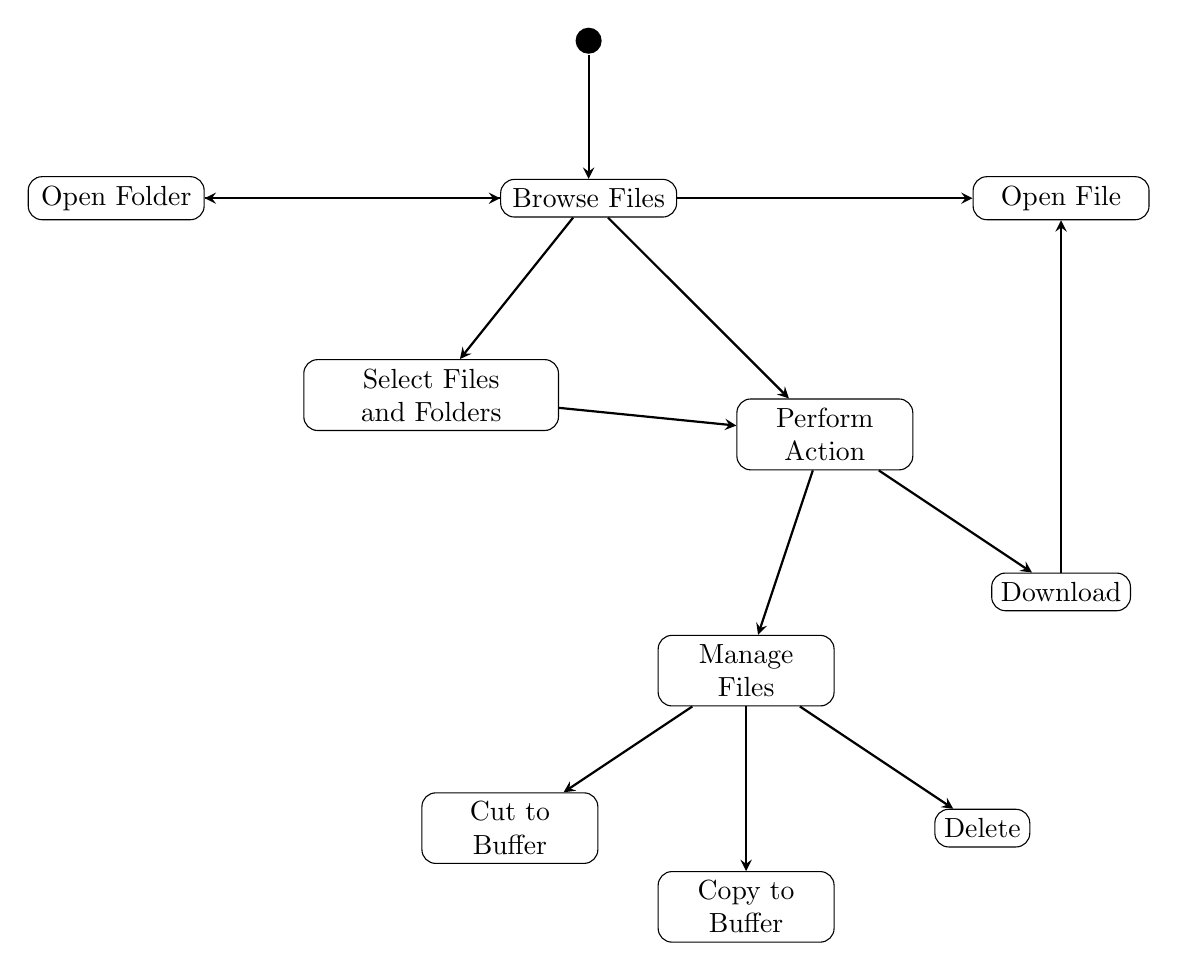
\begin{tikzpicture}[
		node distance=2cm,
		arrow/.style={thick,->,>=stealth},
		start/.style={fill=black,circle,thick},
		label/.style={rectangle, rounded corners=5, text centered, draw=black},
		fixlabel/.style={label, text width=2cm}
	]
	\node[start] at (0, 0) (start) {};
	\node[fixlabel] at (0, -2) (browse) {Browse Files};
	\node[fixlabel] at (-6, -2) (ofolder) {Open Folder};
	\node[fixlabel] at (6, -2) (ofile) {Open File};
	\node[label, text width=3cm] at (-2, -4.5) (select) {Select Files and Folders};
	\node[fixlabel] at (3, -5) (action) {Perform Action};
	\node[label] at (6, -7) (download) {Download};
	\node[fixlabel] at (2, -8) (manage) {Manage Files};
	\node[fixlabel] at (-1, -10) (cut) {Cut to Buffer};
	\node[fixlabel] at (2, -11) (copy) {Copy to Buffer};
	\node[label] at (5, -10) (delete) {Delete};

	\draw[arrow] (start) -- (browse);
	\draw[arrow] (browse) -- (ofile);
	\draw[arrow] (browse) -- (ofolder);
	\draw[arrow] (ofolder) -- (browse);
	\draw[arrow] (browse) -- (select);
	\draw[arrow] (browse) -- (action);
	\draw[arrow] (select) -- (action);
	\draw[arrow] (action) -- (manage);
	\draw[arrow] (action) -- (download);
	\draw[arrow] (download) -- (ofile);
	\draw[arrow] (manage) -- (cut);
	\draw[arrow] (manage) -- (copy);
	\draw[arrow] (manage) -- (delete);
\end{tikzpicture}
\end{center}
\vfill


\section{Database}
\vfill
\begin{center}
Representation of File Metadata in File System. \\
\bigskip
\begin{tabular}{ | m{4cm} | m{3cm} | m{3cm} | m{3cm} | }
	\hline
	\thead{Attribute} &
	\thead{DataType} &
	\thead{Size} &
	\thead{Retrieval} \\
	\hline\hline
	Name               & Chars    & 255 Bytes & Primary Key \\
	Permissions        & Octal    & 4 Bytes   & Not Null \\
	User UID           & Integer  & 4 Bytes   & Not Null \\
	Group GID          & Integer  & 4 Bytes   & Not Null \\
	Modification Time  & Time     & 4 Bytes   & Not Null \\ \hline
\end{tabular}
\end{center}
\vfill


% \section{Gantt Chart}
% \vfill
% \begin{center}
% \begin{ganttchart}[
% 		hgrid=true,
% 		vgrid={*2{dotted}, {dashed}, *3{dotted}, {dashed}, *4{dotted}, {dashed}},
% 		y unit chart=0.8cm,
% 		title height=1,
% 		expand chart=\textwidth,
% 		bar label node/.append style={align=right},
% 		bar height=0.5,
% 		exed/.style={bar top shift=0.5},
% 		real/.style={bar top shift=0.1, bar/.append style={fill=black}},
% 	]{1}{15}
% 	\gantttitle{2024}{15} \ganttnewline[draw=none]
% 	\gantttitle{June}{3}
% 	\gantttitle{July}{4}
% 	\gantttitle{August}{5}
% 	\gantttitle{September}{3} \\
% 	\gantttitlelist{1,...,3}{1}
% 	\gantttitlelist{1,...,4}{1}
% 	\gantttitlelist{1,...,5}{1}
% 	\gantttitlelist{1,...,3}{1} \\
% 	\ganttbar[exed]{Requirements \\ Specification}{1}{1} \\
% 	\ganttbar[real]{}{1}{2} \\
% 	\ganttbar[exed]{Analysis}{2}{3} \\
% 	\ganttbar[real]{}{3}{4} \\
% 	\ganttbar[exed]{Design}{4}{5} \\
% 	\ganttbar[real]{}{5}{7} \\
% 	\ganttbar[exed]{Coding and \\ Testing}{6}{11} \\
% 	\ganttbar[real]{}{8}{12} \\
% 	\ganttbar[exed]{Implementation}{12}{13} \\
% 	\ganttbar[real]{}{13}{15} \\
% \end{ganttchart}
% \end{center}
% \vfill

\fi


\section{System Implementation}


\section{Results}


\section{Conclusion}


\section{References}


\end{document}

